\section{Grundlagen}

Dieses Kapitel führt detailliert in die Robotic Process Automation ein und zeigt die Vorteile dieser Automatisierungsmethode auf. Zudem werden verwandte Arbeiten vorgestellt, die sich mit den Themen der Robotermodellierung in bekannten Notationen oder der einheitlichen Speicherung von Robotermodellen befassen.

\subsection{Einleitung zur Robotic Process Automation}


In den vergangenen Jahrzehnten wurde das Workflow Management angewendet, um Arbeitsabläufe computergestützt zu automatisieren \cite{Aalst2004}. Ein großes Problem bei der Einführung des Workflow Managements stellt die meist mangelhafte Akzeptanz der Mitarbeiter dar. Ebenso lassen sich vollständige Automatisierungen nur schwer in bestehende Systeme integrieren. Um diesen Problemen vorzubeugen, wird das Workflow Management seit einigen Jahren um das Business Process Management (BPM) ergänzt \cite{Aalst2021}. BPM legt den Schwerpunkt auf die von den Mitarbeitern ausgeführen Aufgaben und ermöglicht durch die verwendete Notation BPMN eine vereinfachte Analyse und Optimierung des Prozesses. Da die Mitarbeitenden bei den Automatisierungen nun stärker im Fokus stehen, steigt die Akzeptanz derer bei der Einführung der Automatisierungslösung. Jedoch wird der BPMN vorgeworfen, durch den verstärkten Einsatz der Modellierung den zu automatisierenden Prozess aus dem Fokus zu verlieren. \glqq Schlussendlich ist das Ziel nicht die Modellierung, sondern die Verbesserung des existierenden Prozesses\grqq{} \cite{Aalst2004}.

Um dem meist kostspieligen BPM mit den genannten Nachteilen entgegenzuwirken, wird seit einigen Jahren die Robotic Process Automation entwickelt. Sie wurde anfangs von Wirtschaftsunternehmen vorangetrieben und gerät nun seit vielen Jahren in den Fokus der Wissenschaft \cite{AalstProcessMining}. Ziel der RPA ist es, die vom Nutzer in Drittanwendungen ausgeführten Schritte zu erkennen, aufzuzeichnen und nachfolgend automatisiert auszuführen. Dabei interagiert der sogenannte Softwareroboter analog zum Nutzer mit der grafischen Oberfläche der Software. Da RPA direkt auf dieser Anwendungsebene arbeitet, fällt der Integrationsaufwand im Vergleich zu anderen Automatisierungsmethoden deutlich geringer aus. Es kann weiterhin die bestehende Software genutzt werden, es müssen keine offenen Schnittstellen entwickelt oder gar neue Hardware angeschafft werden. Zwingend notwendig sind jedoch eindeutig definierte Aufgabenfolgen. So lassen sich mittels RPA zum Beispiel Formulare ausfüllen, Daten verschieben, Mails versenden aber auch Informationen von Webseiten verarbeiten. 

RPA ist eine weltweit bekannte Technologie und wird bereits in zwei Dritteln der deutschen Unternehmen verwendet \cite{isgRPA} \cite{pwcRPA}. Zudem ist die RPA mit 63~\% Wachstum in 2018 das am schnellsten wachsende Segment der Softwareentwicklung \cite{gartner}. Ebenso zeichnet sich die Technologie durch eine schnelle Kapitalrendite aus, die vor allem durch den Bottom-Up Ansatz begründet wird. \glqq Oftmals werden die vollständigen Prozesse betrachtet, jedoch nur kleinere Gruppen von Aufgaben - die sogenannten \frqq Quick-wins\flqq - direkt automatisiert \cite{aalstYoutube}.\grqq{} Dies ist nur dadurch möglich, da die Roboter „Hand-in-Hand“ mit den Anwendern arbeiten. 

Wie eingangs beschrieben, unterstützt BPM das Workflow Management bei der Prozessoptimierung. Zur Verbesserung der bestehenden Prozesse wird im Vorfeld einer Robotic Process Automation das Process Mining verwendet. Process Mining analysiert Geschäftsprozesse durch das Verarbeiten und Korrelieren von Datenströmen. Es erkennt Muster in den Prozessdaten und hilft somit das Verständnis der Prozesse zu verbessern. Dadurch lassen sich Möglichkeiten für die sinnvolle Einbindung von RPA erkennen. Vor der Implementierung einer RPA-Lösung empfiehlt sich eine Analyse des umzusetzenden Prozesses mittels Process Mining, da andernfalls der Prozess zwar automatisiert, jedoch vorher nicht optimiert wird. 

Bekannte RPA-Plattformen entwickeln unter anderem die Firmen \mbox{UiPath}\footnote{https://www.uipath.com/de/ (Abgerufen 12. Juni 2021)}, \mbox{blueprism}\footnote{https://www.blueprism.com/de/ (Abgerufen 12. Juni 2021)} und \mbox{AutomationAnywhere}\footnote{https://www.automationanywhere.com/de/ (Abgerufen 12. Juni 2021)}. Die Firma Microsoft stellt mit \code{Power Automate Desktop} seit März 2021 ihre eigene kostenlose RPA-Plattform zur Verfügung. Einige der Plattformen - wie zum Beispiel UiPath - besitzen ein ausgeprägtes \code{Recoding-Feature}, mit dem die zu automatisierenden Aufgaben direkt aufgenommen werden können. Andere hingegen lassen sich  einfacher bedienen oder unterstützen eine Vielzahl an Drittanwendungen. 

\subsection{Einleitung zu Modellierungssprachen}

Um Organisationsstrukturen, Software aber auch Prozesse zu skizzieren, werden zur Beschreibung der Sachverhalte visuelle Modellierungssprachen verwendet \cite{winter2000}. \glqq Neben der Unterstützung bei der Erfassung und Dokumentation sind diese graphischen und textuellen Beschreibungsmittel auch wesentliche Hilfsmittel zur Kommunikation bei der (Weiter-) Entwicklung von Organisationen und Softwaresystemen\grqq{}, beschreibt A. Winter den Nutzen von Modellierungssprachen treffend. Modellierungssprachen unterscheiden sich in dem zur Verfügung gestellten „Vokabular und der Grammatik“, mit der Sachverhalte der menschlich wahrgenommenen Realität in Modellen abgebildet werden können \cite{Fleischmann2018}.

In der durch die Object Management Group (OMG) standardisierten Unified Modeling Language (UML) ist eine Sammlung von Notationen definiert. Die UML umfasst unter anderem das in der Objektmodellierung bekannte Klassendiagramm, das für die Funktionsmodellierung genutzte Use Case Diagramm oder auch das Komponentendiagramm zur Beschreibung von IT-Systemstrukturen. Für dieses Werk von Relevanz sind  die Notationen zur Prozessmodellierung. Diese Sprachen dienen der Darstellung von Interaktionsschritten innerhalb eines Prozesses und eignen sich daher unter Umständen auch zur Modellierung von RPA-Robotern. Bekannte Vertreter sind hierbei das Datenfluss-orientierte Flussdiagramm, die Kontrollfluss-orientierten Sprachen wie die BPMN, das Petri-Netz oder auch die ereignisgesteuerte Prozesskette \cite{mastersthesisLobe}.

\subsection{Verwandte Arbeiten}

In der bestehenden Literatur sind nur wenige Ansätze von Untersuchungen oder Prototypen für die Erstellung von RPA-Robotern in Modellierungssprachen zu finden. Dies ist sehr verwunderlich, da zahlreiche Artikel \cite{alejandro}\cite{rpameetsbpmn} die Wichtigkeit der Dokumentation und Prozessanalyse im Zusammenspiel mit RPA erwähnen.

\clearpage

Eine interessante Arbeit ist womöglich die Abschlussarbeit des Studenten Johann Schäfer der FH Münster \cite{Viadee}. Leider erhielt ich auch nach mehreren Kontaktversuchen keine Antwort auf die Anfrage, die Abschlussarbeit oder vielleicht sogar das Softwareprojekt betrachten zu dürfen. Daher war eine qualitative Analyse sowie eine aufbauende Forschung auf den Erkenntnissen der Arbeit des Studenten nicht möglich.

Der Autor beschreibt eine Weiterentwicklung des \code{bpmn-io} BPMN-Modelers, die sich zum Erstellen von RPA-Robotern eignen soll. Wie in Abbildung \ref{fig:viadee} zu sehen, ist es möglich, mit der entstandenen Plattform jeder BPMN Service Task eine RPA-Aufgabe zuzuweisen. In den grünen Boxen unterhalb der Task ist es möglich, der Aufgabe Parameter zu übergeben. Zudem wird ein aufklappbarer Subprozess verwendet, um auch kleinteilige Automatisierungsschritte übersichtlich darzustellen. Im Hauptprozess (oben dargestellt) ist durch die Annotation direkt erkenntlich, welche Teile des Prozesses mittels RPA automatisiert werden.

\begin{figure}[h!]
    \centering
    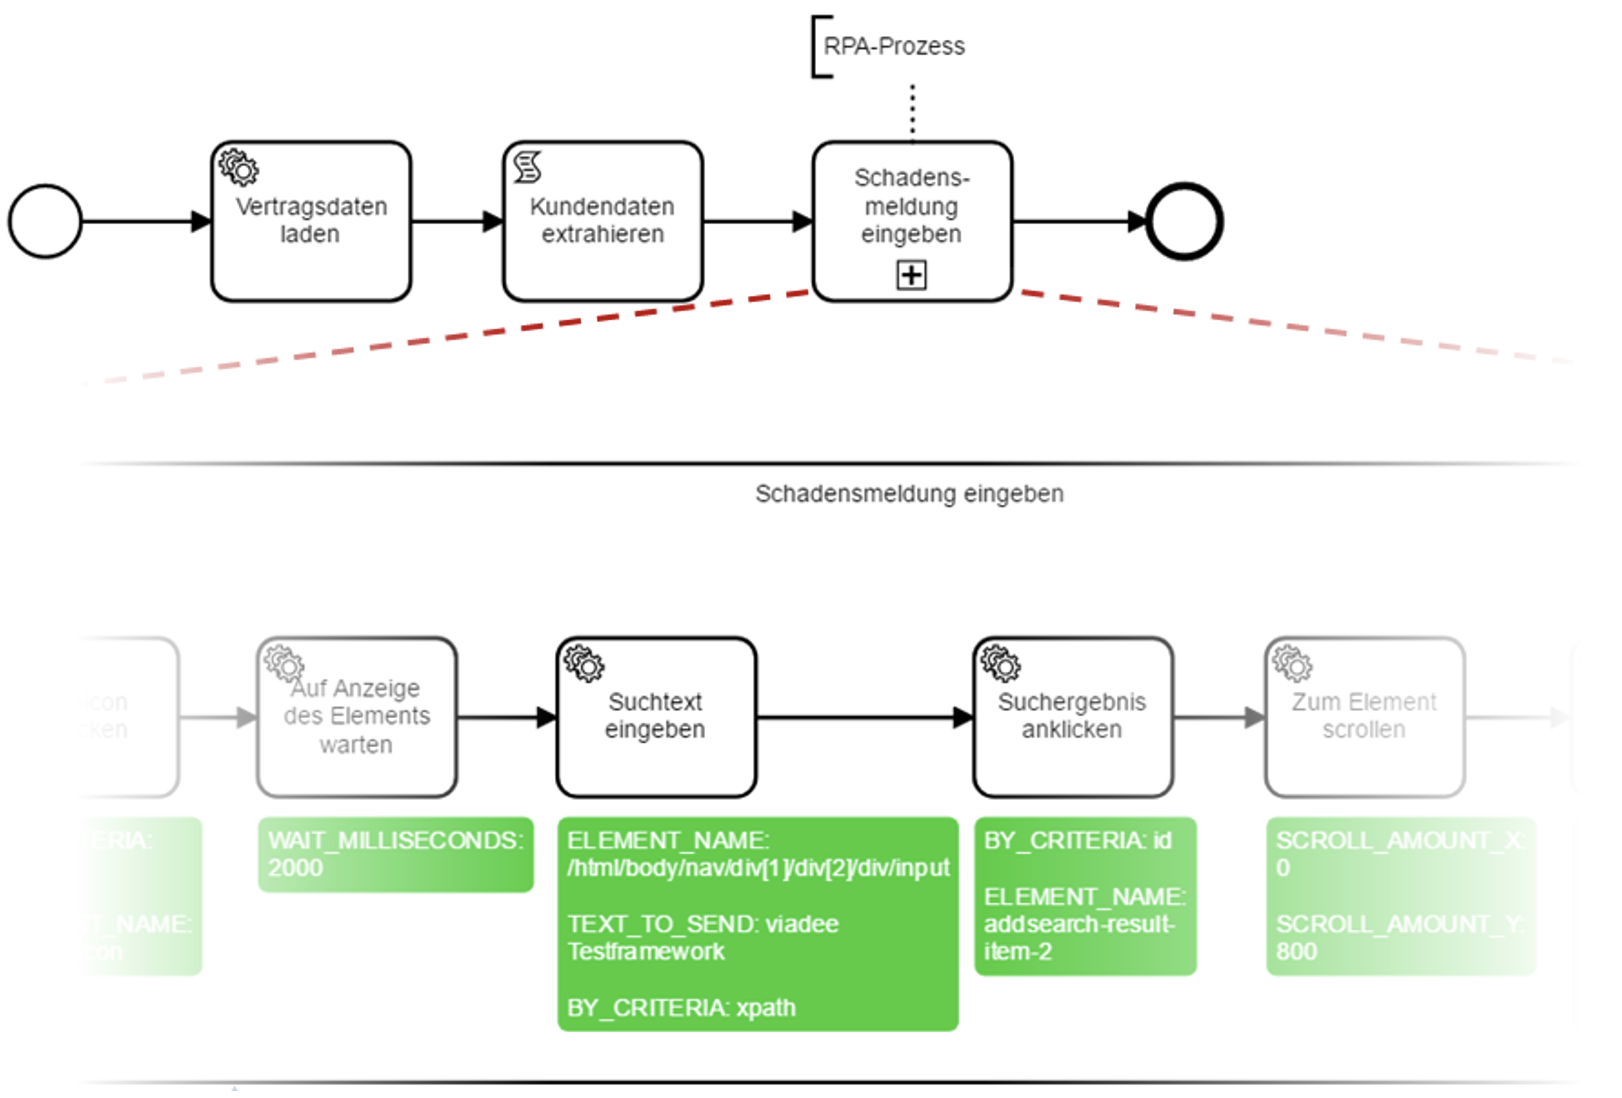
\includegraphics[width=1.0\textwidth]{Bachelorarbeit/images/ScreenshotRelatedWork3.png}
    \caption{Screenshot der Modellierungsoberfläche des viadee-Roboters}
    \label{fig:viadee}
\end{figure}
